\subsection{Precision sensitivity on the OpenAI datasets}
\label{sec:7-precision}

Using FP32 in place of TF32 reduces throughput by about 5\% at matched
configurations, while the checked FP32 frontiers retain their lead over
CAGRA fp32. Source inspection found that the main implementation uses
TF32 multiplication with FP32 accumulation for OpenAI rotation and
centroid matrix products (\cref{sec:4-2}). The precision check
changes that arithmetic switch and alternates the two variants across
probe settings: 37 OpenAI-1536 and 39 OpenAI-3072 configurations, five
rounds each at batch 1,000. Both reuse one TF32-trained model; add and
query arithmetic, including encoding and routing, change. This is not
independent FP32 retraining.

\par\medskip\noindent\begin{minipage}{\linewidth}
\centering\captionsetup{hypcap=false}
\captionof{table}[FP32 sensitivity at matched configurations]{FP32 sensitivity. QPS ratio is FP32/TF32 at equal configuration
(geometric mean); recall differences have the same direction. The last
two columns compare the FP32 frontier at recall 0.97 with archived
IVF-RaBitQ and CAGRA fp32 frontiers. The precision check reuses baseline measurements from the main comparison.}
\label{tab:7-precision}
\scriptsize\setlength{\tabcolsep}{3pt}
\begin{tabular}{@{}lrrrrr@{}}
\toprule
Dataset & Pairs & QPS ratio & $\Delta$Recall & vs RaBitQ & vs CAGRA \\
\midrule
OpenAI-1536 & 37 & 0.953 & +0.0003--+0.0005 & 1.086 & 1.679 \\
OpenAI-3072 & 39 & 0.951 & +0.0000--+0.0003 & 1.079 & 1.629 \\
\bottomrule
\end{tabular}

\end{minipage}\par\medskip

At matched configuration, recall increases by 0--0.0005. At recall 0.97,
FP32 is about 3\% slower than TF32 measured alongside it, but its ratios
to archived RaBitQ are 1.086 on OpenAI-1536 and 1.079 on OpenAI-3072;
ratios to archived CAGRA fp32 are 1.679 and 1.629. The repeated original
variant gives RaBitQ ratios of 1.118 and 1.114, compared with historical
1.130 and 1.157. \Cref{fig:7-precision} shows this paired precision
comparison; the next check remeasures the baselines.

\par\medskip\noindent\begin{minipage}{\linewidth}
\captionsetup{hypcap=false}
\centering
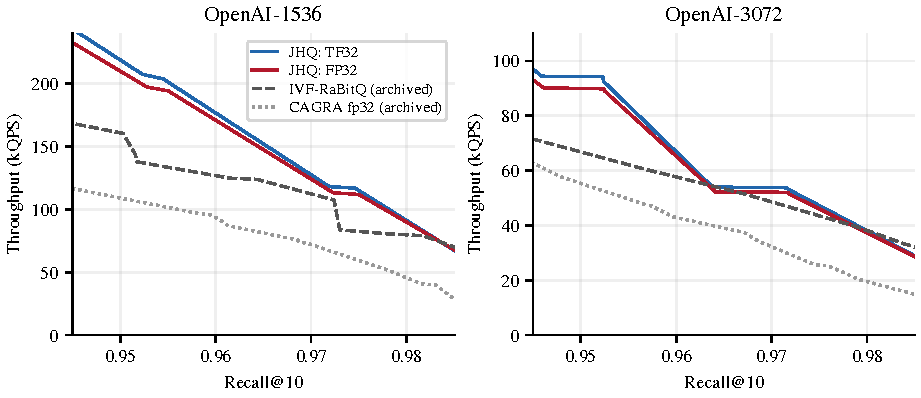
\includegraphics[width=\linewidth]{variants/thesis2/figures/precision.pdf}
\captionof{figure}[TF32 and FP32 precision frontiers]{Precision check. Solid curves are JHQ variants measured together;
dashed/dotted baselines come from the main comparison.
All use the chapter's frontier and interpolation rules.}
\label{fig:7-precision}
\end{minipage}\par\medskip

\subsection{Baselines remeasured with JHQ}
\label{sec:b-precision-anchors}

The same-session check confirms an FP32 lead at recall 0.97 under
both estimators in its tested grid. \Cref{tab:b-precision-anchors}
reports ratios to both RaBitQ and CAGRA fp32.

Twelve paired configurations per OpenAI dataset use the main
comparison's memory-pool settings. Two five-round JHQ repetitions
bracket the baseline runs, and their median rates are combined
geometrically. Equal-configuration FP32/TF32 means are 0.956 for
OpenAI-1536 and 0.964 for OpenAI-3072. Both variants reuse TF32-trained
caches and change only add/query arithmetic.

\par\medskip\noindent\begin{minipage}{\linewidth}
\captionsetup{hypcap=false}
\centering
\captionof{table}[Baselines remeasured with JHQ]{The same-session check at recall 0.97, batch 1,000. Baseline ratios are interpolation / strict measured threshold; FP32/TF32 is interpolated. All methods were remeasured together; the precision check instead reuses the main comparison's baselines.}
\label{tab:b-precision-anchors}
\footnotesize\setlength{\tabcolsep}{3pt}
\begin{tabular}{@{}lrrr@{}}
\toprule
Dataset & FP32/TF32 at 0.97 & FP32 / RaBitQ & FP32 / CAGRA \\
\midrule
OpenAI-1536 & 0.980 & 1.126 / 1.053 & 1.752 / 1.633 \\
OpenAI-3072 & 0.973 & 1.328 / 1.316 & 1.825 / 2.019 \\
\bottomrule
\end{tabular}

\end{minipage}\par\medskip

The check covers a limited grid near recall 0.97. OpenAI-3072's RaBitQ
bracket spans recall 0.9669--0.9796, so the size of the margin depends
on grid coverage and estimator. It is evidence for this local comparison,
not for independently FP32-trained frontiers or every recall target.
